\documentclass[tikz,border=2pt]{standalone}
\usepackage[T1]{fontenc}
\usepackage{amsmath}
\usetikzlibrary{arrows.meta}
\definecolor{rotation}{RGB}{47,83,112}
\begin{document}
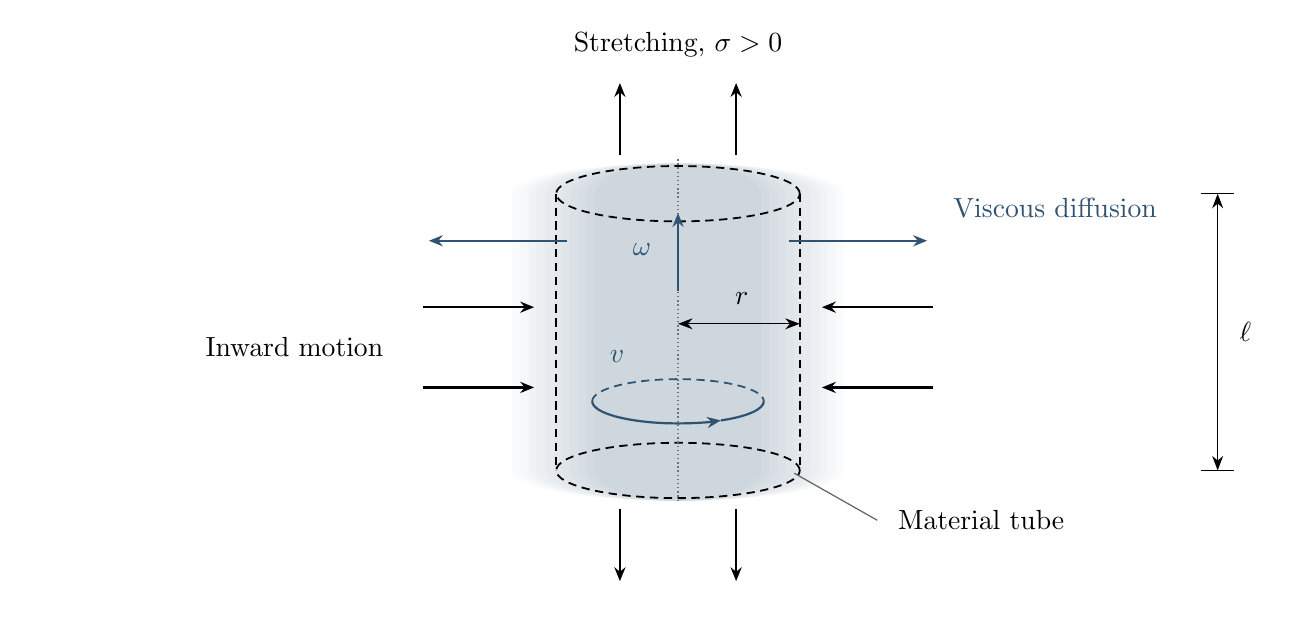
\begin{tikzpicture}[x=1pt,y=1pt,font=\fontsize{10}{12}\selectfont,
 flow/.style={-{Stealth[length=5pt,width=4pt]},line width=.8pt},
 diffusion/.style={flow,rotation},
 dimension/.style={<->,>=Stealth,line width=.5pt}]
 \path[use as bounding box] (0,0) rectangle (448,210);

 % Rotation is concentrated inside and diffuses beyond the material boundary.
 \foreach \R in {60,57,...,30}{
  \path[fill=rotation,fill opacity=.022,draw=none]
   ({235-\R},50) -- ({235-\R},150)
   arc[start angle=180,end angle=0,x radius=\R,y radius=11]
   -- ({235+\R},50)
   arc[start angle=0,end angle=-180,x radius=\R,y radius=11] -- cycle;
 }

 % The dashed contour follows the selected fluid particles.
 \draw[densely dashed,line width=.65pt] (191,150)--(191,50);
 \draw[densely dashed,line width=.65pt] (279,150)--(279,50);
 \draw[densely dashed,line width=.65pt] (235,150) ellipse[x radius=44,y radius=10];
 \draw[densely dashed,line width=.65pt] (235,50) ellipse[x radius=44,y radius=10];
 \draw[densely dotted,black!55,line width=.5pt] (235,39)--(235,163);

 % Axial strain and radial particle motion surround the tube.
 \foreach \x in {214,256}{
  \draw[flow] (\x,164)--(\x,190);
  \draw[flow] (\x,36)--(\x,10);
 }
 \node at (235,204) {Stretching, \(\sigma>0\)};
 \foreach \y in {80,109}{
  \draw[flow] (143,\y)--(183,\y);
  \draw[flow] (327,\y)--(287,\y);
 }
 \node[anchor=east,align=right] at (132,94.5) {Inward motion};

 % Two outward arrows describe one diffusion process.
 \draw[diffusion] (195,133)--(145,133);
 \draw[diffusion] (275,133)--(325,133);
 \node[rotation,anchor=west] at (331,145) {Viscous diffusion};

 % Axial vorticity and circumferential velocity have distinct directions.
 \draw[diffusion,line width=1pt] (235,115)--(235,143);
 \node[rotation] at (222,130) {\(\omega\)};
 \draw[rotation,densely dashed,line width=.65pt]
  (204,75) arc[start angle=180,end angle=0,x radius=31,y radius=8];
 \draw[diffusion]
  (204,75) arc[start angle=180,end angle=300,x radius=31,y radius=8];
 \draw[rotation,line width=.8pt]
  (250.5,68.0718) arc[start angle=300,end angle=360,x radius=31,y radius=8];
 \node[rotation] at (213,91) {\(v\)};

 % Dimensions refer to the material tube.
 \draw[dimension] (235,103)--(279,103);
 \node at (258,112) {\(r\)};
 \draw[dimension] (430,50)--(430,150);
 \draw[line width=.5pt] (424,50)--(436,50);
 \draw[line width=.5pt] (424,150)--(436,150);
 \node at (440,100) {\(\ell\)};
 \draw[black!60,line width=.45pt] (307,32)--(277,49);
 \node[anchor=west] at (311,32) {Material tube};
\end{tikzpicture}
\end{document}
